\documentclass{beamer}
%\documentclass[handout]{beamer} % set this to remove pause breaks
\usetheme{McMaster}
\usepackage{cancel}
\title{omg wtf twitter}
\author{John Fink}
\date{November 25, 2022}
\begin{document}
\begin{frame}[plain]
    \maketitle
\end{frame}
\begin{frame}{A Brief History of (some of) Twitter}
	\begin{itemize}
		\pause
		\item 2004: TXTmob
		\pause
		\item 2006: Twttr, an Odeo side project
		\pause
		\item 2007: Twitter gets \$100k venture investment
		\pause
		\item 2009: Twitter featured on Oprah
		\pause
		\item 2011: Twitter and the Arab Spring
		\pause
		\item 2013: Twitter goes public
		\pause 
		\item 2015: Twitter unprofitable
		\pause
		\item 2017: Twitter profitable?
		\pause
		\item 2022: Elon Musk proposes buying twitter at \$54.20 a share, approximately \$44 billion dollars in total.
	\end{itemize}
\end{frame}

\begin{frame}{\$54.20 a share}
	\begin{itemize}
		\pause
		\item .20c extra per share
		\pause
		\item .20c extra per share x 765 million outstanding shares
		\pause
		\item .20c extra per share x 765 million outstanding shares = \$153m
		\pause
		\item Elon Musk spends \$153m for a dumb weed joke
		\pause 
		\item Elon Musk owes \$1 \textbf{billion} in \textbf{interest} each year.
	\end{itemize}	
\end{frame}


\begin{frame}{A Brief History of November 2022}
	\begin{itemize}
		\pause
		\item Late Oct: Elon Musk purchases Twitter
		\pause
		\item Nov 4: Thousands of employees are laid off
		\pause
		\item Nov 9: New Twitter Blue
	\end{itemize}
\end{frame}
\begin{frame}
	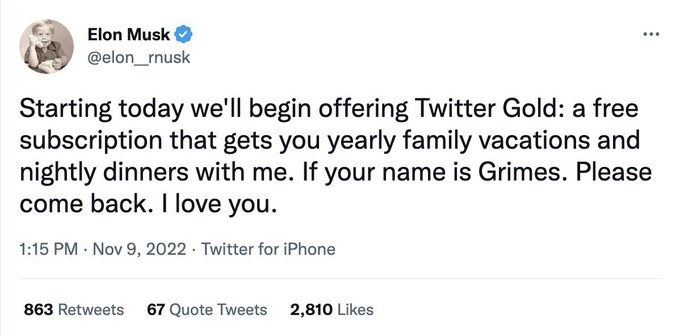
\includegraphics[width = \textwidth]{twitter-gold}
\end{frame}

\begin{frame}
	
\includegraphics[height = \textheight]{itsame}
\end{frame}

\begin{frame}
	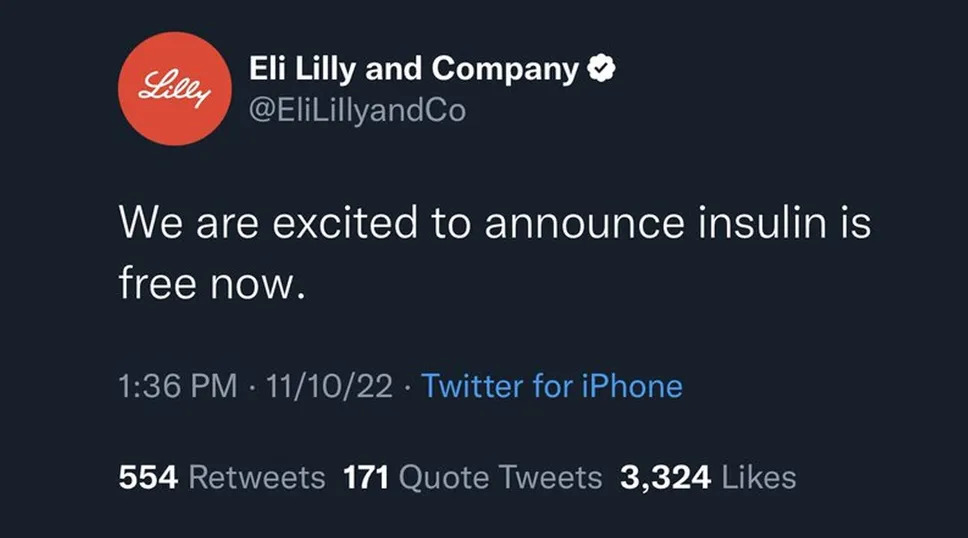
\includegraphics[width = \textwidth]{free-insulin}
\end{frame}

\begin{frame}
	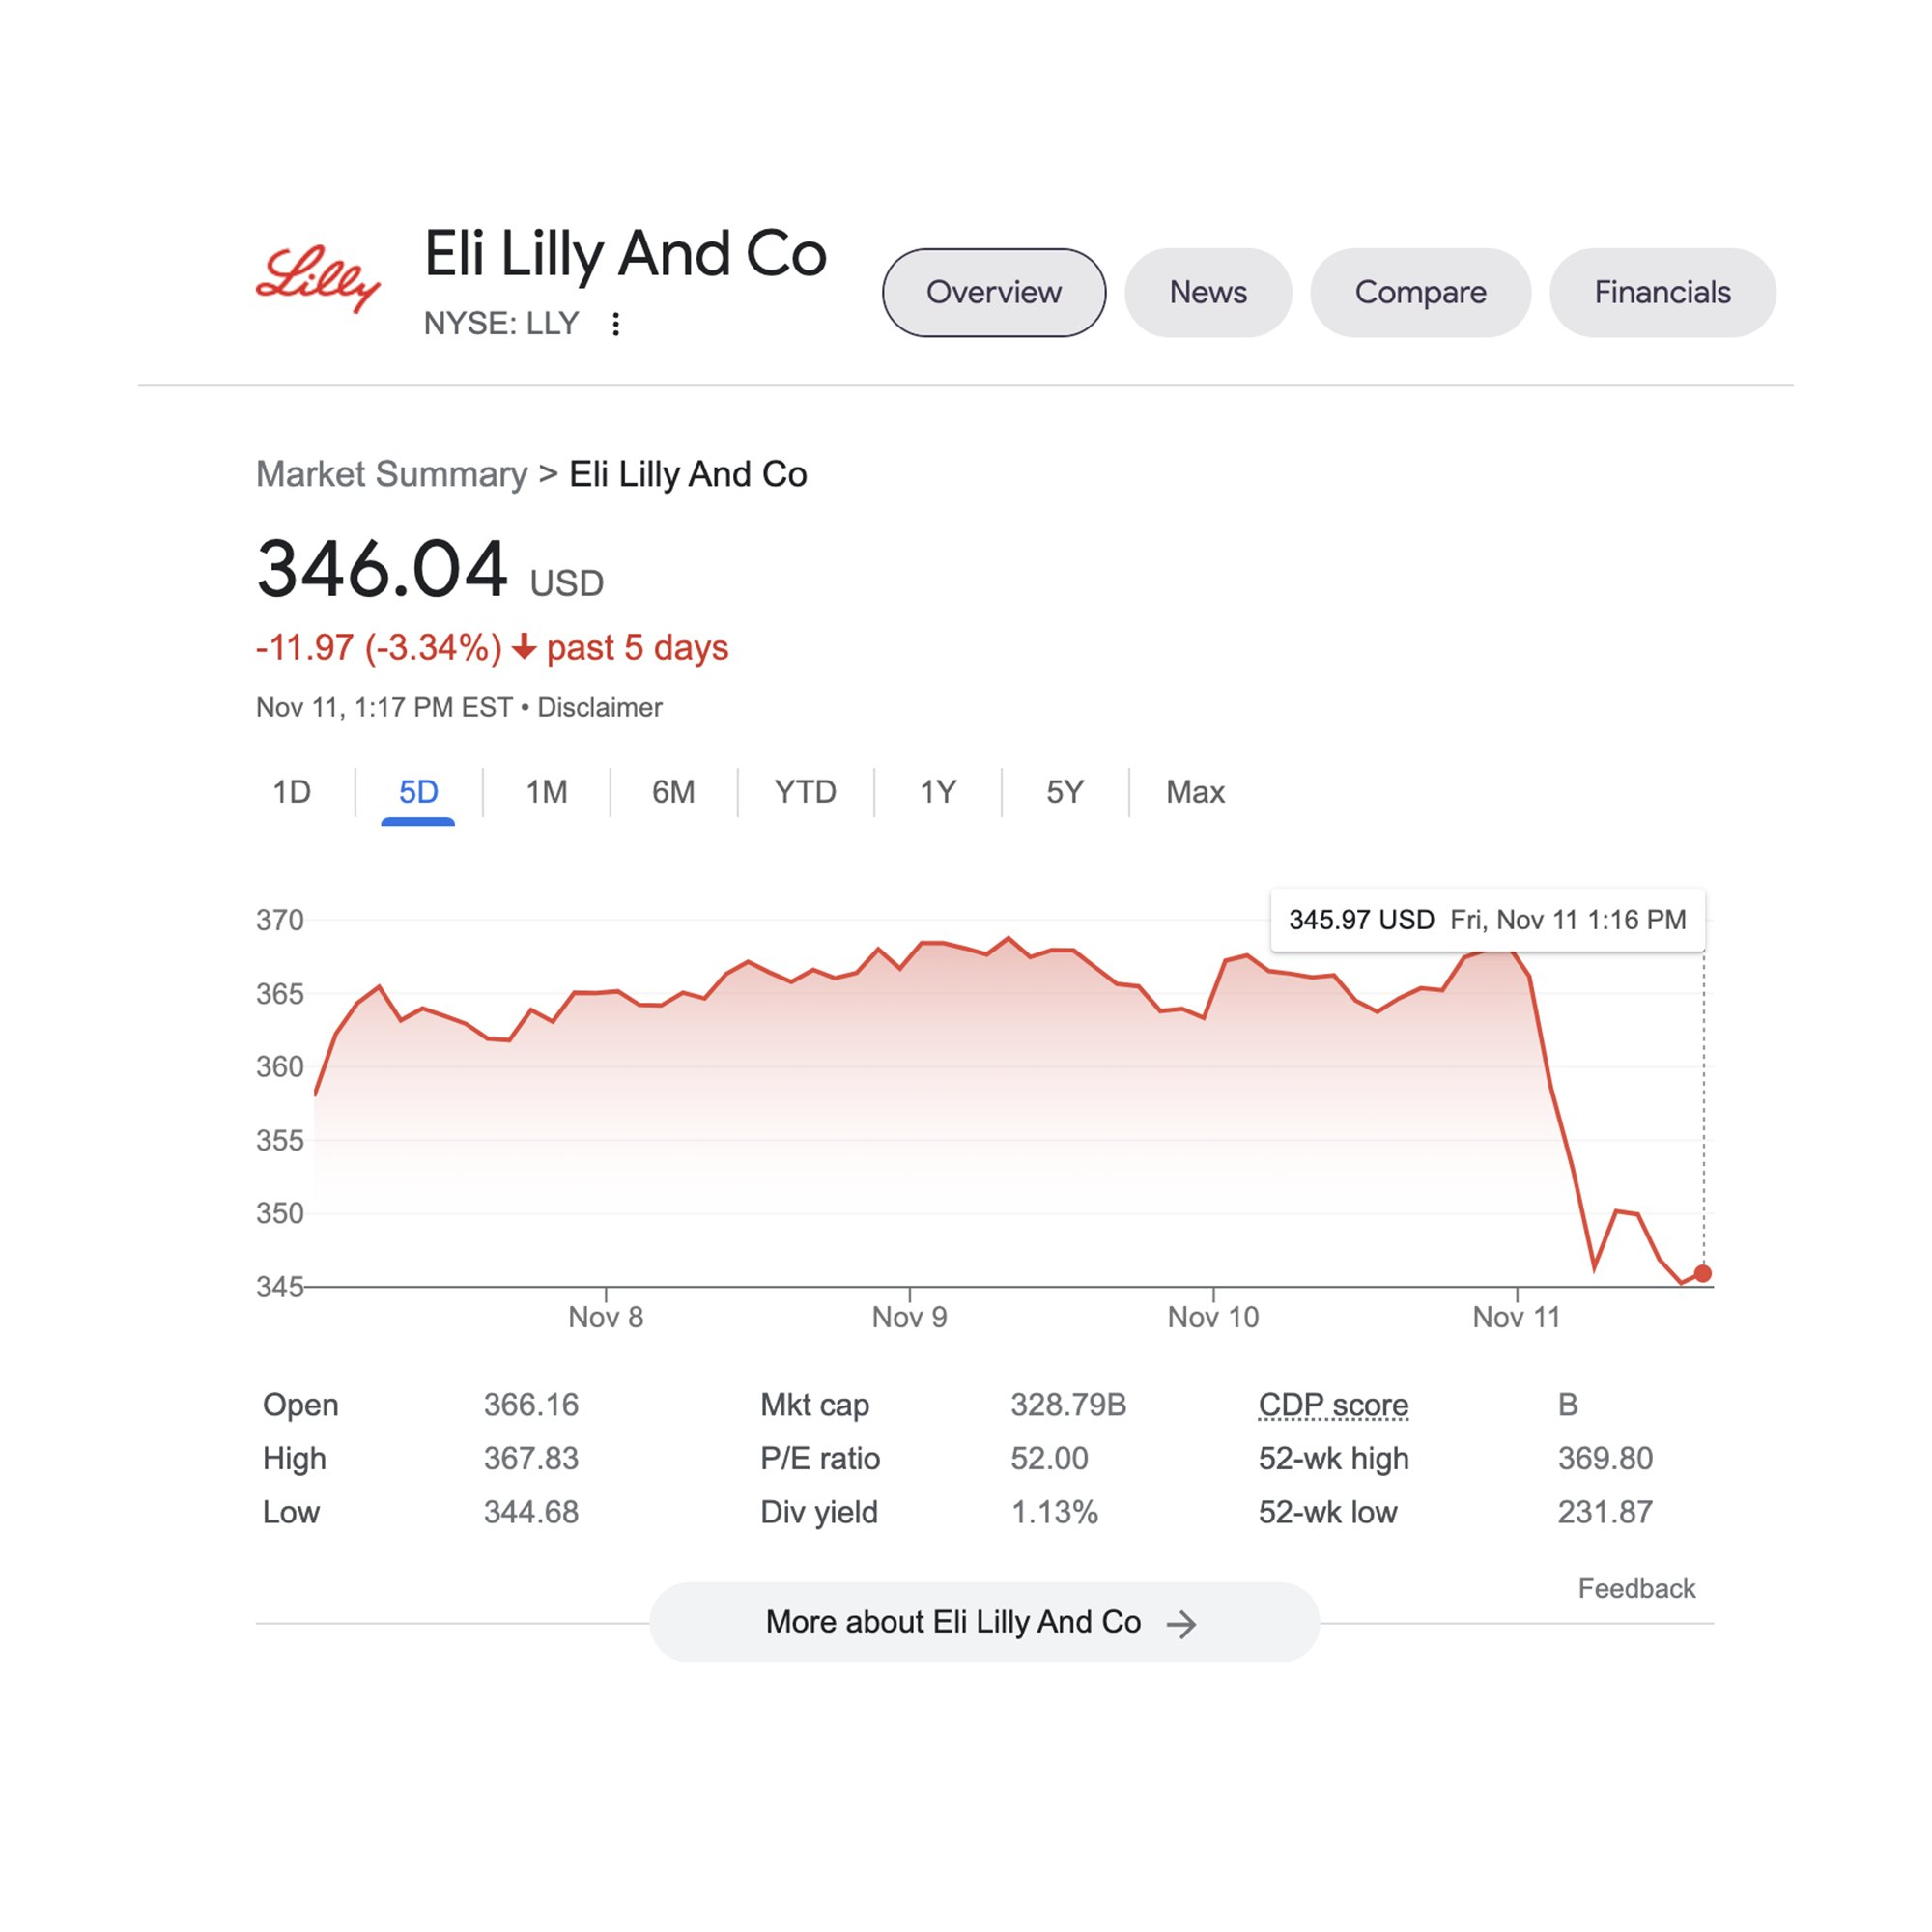
\includegraphics[width = \textwidth]{eli-lilly-stock}
\end{frame}

\begin{frame}{A Brief History of November 2022}
	\begin{itemize}
	\item Late Oct: Elon Musk purchases Twitter
	\item Nov 4: Thousands of employees are laid off
	\item Nov 9: New Twitter Blue
	\pause
	\item Nov 10: Trust and Safety sickout
	\pause
	\item Nov 11: Twitter employees personally responsible for FTC compliance
	\pause
	\item Nov 22: Trump reinstated
	\pause
	\item Nov 23: 50\% of top 100 advertisers have suspended activity
	\pause
	\item Nov 24: Amnesty for suspended accounts	
	
	\end{itemize}
\end{frame}

\begin{frame}{Current state of Twitter}
	It's a little bit difficult to tell for sure but it appears that Twitter has \textbf{no} or \textbf{greatly diminished}:
	\begin{itemize}
		\pause
		\item Comms department
		\pause
		\item Moderation team
		\pause
		\item International groups (Africa, Canada, Ireland, others?)
		\pause
		\item ....uh GDPR?
		\pause 
		\item Infrastructure team 
		\pause
		\item (this one is important because Twitter infra is *all on prem* and apparently not virtualized/containered)
	\end{itemize}
\end{frame}

\begin{frame}{Disaster Scenario}
	\textbf{Right now} things that still work:
	\begin{itemize}
		\pause
		\item ....tweeting
		\pause
		\item the API
	\end{itemize}
\end{frame}

\begin{frame}{Disaster Scenario}
	User facing things that either \textbf{don't work} or have \textbf{failed} at least once:
	\begin{itemize}
		\pause
		\item 2FA
		\pause
		\item Using Twitter as external auth
		\pause
		\item deplatforming various chuds
	\end{itemize}
\end{frame}

\begin{frame}{About that API}
	The impending loss of Twitter or, more likely, its level of API access necessitates us to face some very unpleasant realities about the ability of academic/non-commercial entities to analyze social media data. As the need for Twitter to generate serious income mounts -- remember that \$1 \textbf{billion} each year just to service the debt -- it's probably a reasonable expectation that services -- especially free ones, like the API -- will degrade or be turned off.
	\newline
	
	Other than Reddit, are there any other major social media websites that enable easy harvesting of data for free or cheap?
\end{frame}

\begin{frame}
	Any questions or comments?
	
	John Fink  (\xcancel{@adr}) / @jbfink@glammr.us / @adr@mastodon.social
\end{frame}

\end{document}
